\documentclass[11pt,a4paper]{beamer}
\usetheme{Madrid} % temas en http://deic.uab.es/~iblanes/beamer_gallery/index_by_theme_and_color.html
\usepackage{latexsym}
\usepackage[utf8]{inputenc}
\usepackage[spanish]{babel}
\usepackage{amsmath, amsfonts, amssymb}
\usepackage{makeidx}
\usepackage{hyperref}
\usepackage{graphicx}
\DeclareGraphicsExtensions{.eps,.pdf,.png}

\setbeamertemplate{navigation symbols}{}

\usefonttheme{professionalfonts}
\setbeamercovered{transparent}

\title[Presentaciones en \LaTeX] 
{Presentaciones en \LaTeX}
\subtitle{Clase Beamer}


\author[Torres M.] % (optional, for multiple authors)
{Torres M.\inst{1} \and España A.\inst{2}}
\institute[EPN] % (optional)
{
  \inst{1}%
  Facultad de Ciencias\\ % Instituto
  Escuela Politécnica Nacional % Universidad
  \and
  \inst{2}%
  Facultad de Ciencias\\
  Escuela Politécnica Nacional
}


\date[2015] % (optional)
{Curso de \LaTeX, 2015}
\subject{Escritura en \LaTeX}

\begin{document}

\begin{frame}  % Diapositiva de Titulo 
\titlepage
\end{frame}

\begin{frame}<beamer> % Diapositiva de Indice
\frametitle{Contenido}
\tableofcontents
\end{frame}

\AtBeginSection  % Diapositiva de inicio de seccion 
{
\begin{frame}
\begin{center}
\begin{beamercolorbox}[sep=8pt,center]{part title}
\usebeamerfont{part title}
\insertsection
\end{beamercolorbox}
\end{center}
\end{frame} 
}

\section{Algunos Ejemplos en  \LaTeX {}} 

\begin{frame}
\frametitle{Campo Galois $GF(p^r)$}
\framesubtitle{Resumen}
\begin{enumerate}
\item Todo dominio integral {\em finito} es un campo \\
\item Si $F$ es un campo con $q$ elementos , y $a$ es un elemento no nulo de $F$,
entonces $a^{q -1}=1$\\
\item Si $F$ es un campo con $q$ elementos , entonces cualquier $a \in \, F$
satisface la ecuación $x^q-x=0$\\
\end{enumerate}
\end{frame}

\begin{frame}
\frametitle{Campo Galois $GF(p^r)$}
\framesubtitle{Resumen}
\begin{enumerate}[<+->]
% <- Nueva opción
\item Sea $F$ un campo con $q$ elementos y $a$ un elemento no
nulo de $F$. Si $n$ es el orden de $a$, entonces $n|(q-1)$.
\item Sea $p$ primo y $m(x)$ un polinomio irreducible de grado $r$ en $Z_p[x]$.
Entonces la clase residual $Z_p[x]/\ equiv _{m(x)}$ es un campo con $p^r$
elementos que contiene $Z_p$ y una raíz de $m(x)$.
\item Sea $F$ un campo con $q$ elementos.
Entonces $q=p^r$ con $p$ primo y $r \in \, N$
\end{enumerate}
\end{frame}

\begin{frame}{Ejemplo}
\begin{enumerate}
\item <1-> $x^4-x=0$
\item <2-> $x(x^3-1) =0$
\item <3-> $x =0 \;$ o $\;x^3 -1=0$
\item <4-> $x =0 \;$ o $\;x=\ sqrt [3]{1}$
\item <1-> $\Longrightarrow x=0,\; x=1$
\end{enumerate}
\end{frame}

\begin{frame}{ Nodos igualmente espaciados}
\begin{block}{ Diferencias hacia adelante}
\begin{eqnarray*}
\Delta^0 y_k&:=&y_k,\\
\Delta^1 y_k&=&y_{k+1}-y_k,\\
\Delta^2 y_k&=&\Delta(y_{k+1}-y_k)\; \\
&=&\;y_{k+2}-y_{k+1}-y_{k+1}+y_k\; \\
&=&\;y_{k+2}-2y_{k+1}+y_k,\\
&\dots &\\
\Delta^n y_k&=&\sum_{j=0}^{n}(-1)^j\binom{n}{j}y_{k+n-j}
\end{eqnarray*}
\end{block}
\end{frame}

 
%muestra la sección de Ejemplos en Tablas y Figuras en la tabla de contenido
 
\subsection{Tablas y Figuras} %muestra la sub-sección Tablas y Figuras en la tabla de contenido
 
\begin{frame}{Tablas y Figuras}
 
\begin{itemize}
\item Utilice \texttt{tabular} para generar itemize simples 
\item Puede cargar una figura (JPEG, PNG o PDF) a través del menú Archivos.
\item Para incluirlo en el documento, utilice el comando \texttt{includegraphics} 
(véase el comentario más adelante en el código fuente).
\end{itemize}
 
 Comandos para incluir una figura:
\begin{figure}
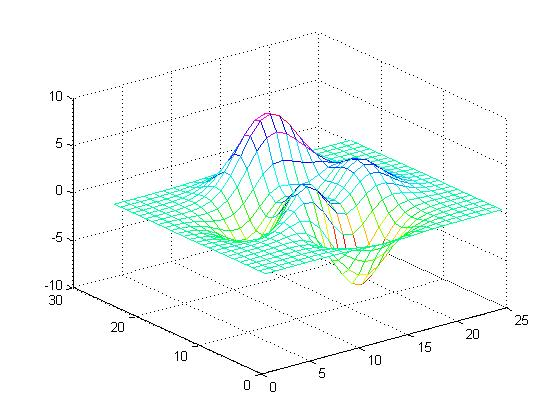
\includegraphics[scale=0.2]{Imagenes/figura1}
\caption{\label{fig:your-figure} Encabezamiento va aqui.}
\end{figure}
 
% Comando  para incluir una tabla simple:
\begin{table}
\centering
\begin{tabular}{l|r}
Articulo & Cantidad \\\hline
Widgets & 42 \\
Gadgets & 13
\end{tabular}
\caption{\label{tab:widgets} Un ejemplo de tabla.}
\end{table}
\end{frame}

\begin{frame}
\frametitle{Mi animación}
\begin{figure}[t]
\centering
\includegraphics<1>[scale=0.5, angle=0]{Imagenes/figura1}
\includegraphics<2>[scale=0.5, angle=30]{Imagenes/figura1}
\includegraphics<3>[scale=0.5, angle=60]{Imagenes/figura1}
\includegraphics<4>[scale=0.5, angle=90]{Imagenes/figura1}
\includegraphics<5>[scale=0.5, angle=120]{Imagenes/figura1}
\includegraphics<6->[scale=0.5, angle=150]{Imagenes/figura1}
\end{figure}
\end{frame}
 
%\begin{frame}%[allowframebreaks]%in case more than 1 slide needed
%	\frametitle{Bibliografía}
%  {
%   \nocite{*}
%    \footnotesize
%  \bibliographystyle{apalike}
%   \bibliography{Bibliografia}
%    }
%\end{frame}

\begin{frame}
\frametitle{Bibliografía}
\begin{thebibliography}{9}
\setbeamertemplate{bibliography item}[online]
\bibitem{A} ItemA
\setbeamertemplate{bibliography item}[book]
\bibitem{B} ItemB
\setbeamertemplate{bibliography item}[article]
\bibitem{C} ItemC
\setbeamertemplate{bibliography item}[triangle]
\bibitem{D} ItemD
\setbeamertemplate{bibliography item}[text]
\bibitem{E} ItemE
\end{thebibliography}
\end{frame}

\end{document}